\PassOptionsToPackage{unicode=true}{hyperref} % options for packages loaded elsewhere
\PassOptionsToPackage{hyphens}{url}
%
\documentclass[
]{article}
\usepackage{lmodern}
\usepackage{amssymb,amsmath}
\usepackage{ifxetex,ifluatex}
\ifnum 0\ifxetex 1\fi\ifluatex 1\fi=0 % if pdftex
  \usepackage[T1]{fontenc}
  \usepackage[utf8]{inputenc}
  \usepackage{textcomp} % provides euro and other symbols
\else % if luatex or xelatex
  \usepackage{unicode-math}
  \defaultfontfeatures{Scale=MatchLowercase}
  \defaultfontfeatures[\rmfamily]{Ligatures=TeX,Scale=1}
\fi
% use upquote if available, for straight quotes in verbatim environments
\IfFileExists{upquote.sty}{\usepackage{upquote}}{}
\IfFileExists{microtype.sty}{% use microtype if available
  \usepackage[]{microtype}
  \UseMicrotypeSet[protrusion]{basicmath} % disable protrusion for tt fonts
}{}
\makeatletter
\@ifundefined{KOMAClassName}{% if non-KOMA class
  \IfFileExists{parskip.sty}{%
    \usepackage{parskip}
  }{% else
    \setlength{\parindent}{0pt}
    \setlength{\parskip}{6pt plus 2pt minus 1pt}}
}{% if KOMA class
  \KOMAoptions{parskip=half}}
\makeatother
\usepackage{xcolor}
\IfFileExists{xurl.sty}{\usepackage{xurl}}{} % add URL line breaks if available
\IfFileExists{bookmark.sty}{\usepackage{bookmark}}{\usepackage{hyperref}}
\hypersetup{
  pdftitle={Assignment 1},
  pdfauthor={Walter Verwer \& Bas Machielsen},
  pdfborder={0 0 0},
  breaklinks=true}
\urlstyle{same}  % don't use monospace font for urls
\usepackage[margin=1in]{geometry}
\usepackage{color}
\usepackage{fancyvrb}
\newcommand{\VerbBar}{|}
\newcommand{\VERB}{\Verb[commandchars=\\\{\}]}
\DefineVerbatimEnvironment{Highlighting}{Verbatim}{commandchars=\\\{\}}
% Add ',fontsize=\small' for more characters per line
\usepackage{framed}
\definecolor{shadecolor}{RGB}{248,248,248}
\newenvironment{Shaded}{\begin{snugshade}}{\end{snugshade}}
\newcommand{\AlertTok}[1]{\textcolor[rgb]{0.94,0.16,0.16}{#1}}
\newcommand{\AnnotationTok}[1]{\textcolor[rgb]{0.56,0.35,0.01}{\textbf{\textit{#1}}}}
\newcommand{\AttributeTok}[1]{\textcolor[rgb]{0.77,0.63,0.00}{#1}}
\newcommand{\BaseNTok}[1]{\textcolor[rgb]{0.00,0.00,0.81}{#1}}
\newcommand{\BuiltInTok}[1]{#1}
\newcommand{\CharTok}[1]{\textcolor[rgb]{0.31,0.60,0.02}{#1}}
\newcommand{\CommentTok}[1]{\textcolor[rgb]{0.56,0.35,0.01}{\textit{#1}}}
\newcommand{\CommentVarTok}[1]{\textcolor[rgb]{0.56,0.35,0.01}{\textbf{\textit{#1}}}}
\newcommand{\ConstantTok}[1]{\textcolor[rgb]{0.00,0.00,0.00}{#1}}
\newcommand{\ControlFlowTok}[1]{\textcolor[rgb]{0.13,0.29,0.53}{\textbf{#1}}}
\newcommand{\DataTypeTok}[1]{\textcolor[rgb]{0.13,0.29,0.53}{#1}}
\newcommand{\DecValTok}[1]{\textcolor[rgb]{0.00,0.00,0.81}{#1}}
\newcommand{\DocumentationTok}[1]{\textcolor[rgb]{0.56,0.35,0.01}{\textbf{\textit{#1}}}}
\newcommand{\ErrorTok}[1]{\textcolor[rgb]{0.64,0.00,0.00}{\textbf{#1}}}
\newcommand{\ExtensionTok}[1]{#1}
\newcommand{\FloatTok}[1]{\textcolor[rgb]{0.00,0.00,0.81}{#1}}
\newcommand{\FunctionTok}[1]{\textcolor[rgb]{0.00,0.00,0.00}{#1}}
\newcommand{\ImportTok}[1]{#1}
\newcommand{\InformationTok}[1]{\textcolor[rgb]{0.56,0.35,0.01}{\textbf{\textit{#1}}}}
\newcommand{\KeywordTok}[1]{\textcolor[rgb]{0.13,0.29,0.53}{\textbf{#1}}}
\newcommand{\NormalTok}[1]{#1}
\newcommand{\OperatorTok}[1]{\textcolor[rgb]{0.81,0.36,0.00}{\textbf{#1}}}
\newcommand{\OtherTok}[1]{\textcolor[rgb]{0.56,0.35,0.01}{#1}}
\newcommand{\PreprocessorTok}[1]{\textcolor[rgb]{0.56,0.35,0.01}{\textit{#1}}}
\newcommand{\RegionMarkerTok}[1]{#1}
\newcommand{\SpecialCharTok}[1]{\textcolor[rgb]{0.00,0.00,0.00}{#1}}
\newcommand{\SpecialStringTok}[1]{\textcolor[rgb]{0.31,0.60,0.02}{#1}}
\newcommand{\StringTok}[1]{\textcolor[rgb]{0.31,0.60,0.02}{#1}}
\newcommand{\VariableTok}[1]{\textcolor[rgb]{0.00,0.00,0.00}{#1}}
\newcommand{\VerbatimStringTok}[1]{\textcolor[rgb]{0.31,0.60,0.02}{#1}}
\newcommand{\WarningTok}[1]{\textcolor[rgb]{0.56,0.35,0.01}{\textbf{\textit{#1}}}}
\usepackage{graphicx,grffile}
\makeatletter
\def\maxwidth{\ifdim\Gin@nat@width>\linewidth\linewidth\else\Gin@nat@width\fi}
\def\maxheight{\ifdim\Gin@nat@height>\textheight\textheight\else\Gin@nat@height\fi}
\makeatother
% Scale images if necessary, so that they will not overflow the page
% margins by default, and it is still possible to overwrite the defaults
% using explicit options in \includegraphics[width, height, ...]{}
\setkeys{Gin}{width=\maxwidth,height=\maxheight,keepaspectratio}
\setlength{\emergencystretch}{3em}  % prevent overfull lines
\providecommand{\tightlist}{%
  \setlength{\itemsep}{0pt}\setlength{\parskip}{0pt}}
\setcounter{secnumdepth}{-2}
% Redefines (sub)paragraphs to behave more like sections
\ifx\paragraph\undefined\else
  \let\oldparagraph\paragraph
  \renewcommand{\paragraph}[1]{\oldparagraph{#1}\mbox{}}
\fi
\ifx\subparagraph\undefined\else
  \let\oldsubparagraph\subparagraph
  \renewcommand{\subparagraph}[1]{\oldsubparagraph{#1}\mbox{}}
\fi

% set default figure placement to htbp
\makeatletter
\def\fps@figure{htbp}
\makeatother


\title{Assignment 1}
\author{Walter Verwer \& Bas Machielsen}
\date{\today}

\begin{document}
\maketitle

\hypertarget{question-1-the-sample-selection-model.}{%
\subsection{Question 1: The sample selection
model.}\label{question-1-the-sample-selection-model.}}

A researcher aims to gain insight in the potential earnings of the
non-employed. (In the data, the non-employed can be identified by a
missing value for the earnings variable). She realizes that the sample
of observed wages may be subject to sample selection.

\textbf{(a) Run an OLS regression for log-earnings on schooling, age,
and age squared. Present the results and comment on the estimates.}

\begin{Shaded}
\begin{Highlighting}[]
\NormalTok{model_}\DecValTok{1}\NormalTok{ <-}\StringTok{ }\KeywordTok{lm}\NormalTok{(}\DataTypeTok{data =}\NormalTok{ data, }\DataTypeTok{formula =}\NormalTok{ logWage }\OperatorTok{~}\StringTok{ }\NormalTok{schooling }\OperatorTok{+}\StringTok{ }\NormalTok{age }\OperatorTok{+}\StringTok{ }\NormalTok{age2)}

\NormalTok{results_}\DecValTok{1}\NormalTok{ <-}\StringTok{ }\KeywordTok{summary.lm}\NormalTok{(model_}\DecValTok{1}\NormalTok{)}
\NormalTok{coeffs_}\DecValTok{1}\NormalTok{ <-}\StringTok{ }\NormalTok{results_}\DecValTok{1}\OperatorTok{$}\NormalTok{coefficients[,}\DecValTok{1}\NormalTok{]}
\NormalTok{pvals_}\DecValTok{1}\NormalTok{ <-}\StringTok{ }\NormalTok{results_}\DecValTok{1}\OperatorTok{$}\NormalTok{coefficients[,}\DecValTok{4}\NormalTok{]}

\KeywordTok{stargazer}\NormalTok{(model_}\DecValTok{1}\NormalTok{, }\DataTypeTok{style =} \StringTok{"AER"}\NormalTok{,}
          \DataTypeTok{font.size =} \StringTok{"small"}\NormalTok{,}
          \DataTypeTok{header =}\NormalTok{ F, }\DataTypeTok{label =} \StringTok{'tab:q1_a_ols'}\NormalTok{,}
          \DataTypeTok{title =} \StringTok{'OLS regression for log-earnings on schooling, age and age squared.'}\NormalTok{)}
\end{Highlighting}
\end{Shaded}

\begin{table}[!htbp] \centering 
  \caption{OLS regression for log-earnings on schooling, age and age squared.} 
  \label{tab:q1_a_ols} 
\small 
\begin{tabular}{@{\extracolsep{5pt}}lc} 
\\[-1.8ex]\hline 
\hline \\[-1.8ex] 
\\[-1.8ex] & logWage \\ 
\hline \\[-1.8ex] 
 schooling & 0.216$^{***}$ \\ 
  & (0.032) \\ 
  & \\ 
 age & $-$0.342 \\ 
  & (0.521) \\ 
  & \\ 
 age2 & $-$0.011 \\ 
  & (0.008) \\ 
  & \\ 
 Constant & 26.400$^{***}$ \\ 
  & (8.060) \\ 
  & \\ 
Observations & 416 \\ 
R$^{2}$ & 0.815 \\ 
Adjusted R$^{2}$ & 0.813 \\ 
Residual Std. Error & 1.500 (df = 412) \\ 
F Statistic & 604.000$^{***}$ (df = 3; 412) \\ 
\hline \\[-1.8ex] 
\textit{Notes:} & \multicolumn{1}{l}{$^{***}$Significant at the 1 percent level.} \\ 
 & \multicolumn{1}{l}{$^{**}$Significant at the 5 percent level.} \\ 
 & \multicolumn{1}{l}{$^{*}$Significant at the 10 percent level.} \\ 
\end{tabular} 
\end{table}

The results show that one additional year of schooling has an effect of
0.216 on log(Wage), which means that one additional year of schooling
has an estimated 21.6\% effect on wages earned. This result is highly
significant (p-value is \ensuremath{2.706\times 10^{-11}}) Another
result, shown in figure \ref{tab:q1_a_ols} is that being one year older
has an estimated effect of -0.342 on log(Wage). Thus, being one year
older is estimated to have a -34.189\% on wages. This result is not
significant at a common level (p-value is 0.512). The third estimated
coefficients is the one corresponding to the variable age squared. It
has an estimated coefficient of -0.011, which represents the estimated
effect of a one unit increase in age squared on log(Wage). This also
means that a one unit increase in age squared is equal to an estimate
effect of -1.114\% on the linear representation of wage. This effect is
not significant at common levels, because the p-value is 0.184. Finally,
the estimated constant in the model is estimated at 26.409. This means
that if all other variables are zero, then the log(Wage) will be equal
to 26.409. Thus, if all other variables are zero, then wage is estimated
to be equal to exp(26.409)=\ensuremath{2.947\times 10^{11}}. This is an
extremely high number given the characteristics of the wage variable.
However, this result is highly significant, because the p-value is
0.001.

\textbf{(b) Briefly discuss the sample selection problem that may arise
in using these OLS estimates for the purpose of predicting the potential
earnings of the non-employed. Formulate the sample selection model. In
your answer, include an explanation why OLS may fail in this context.}

An individual is only in this data set if they earn wages, i.e.~if they
are employed. Being employed itself is not randomly allocated, but
rather, a function of e.g.~age, age\^{}2, and schooling. Also,
employment status follows from labor supply and demand forces. Hence,
the estimates of schooling on earnings are conditional on having
earnings to begin with, whereas unbiased estimates must also include
those individuals. Formally,
\(\mathbb{E}[\text{Earnings}] = \mathbb{E[\text{Earnings}|\text{Having a job}]} \cdot \mathbb{P}[\text{Having a job}] + \mathbb{E[\text{Earnings}|\text{Not having a job}]} \cdot (1-\mathbb{P[\text{Having a job}]})\).
The given estimation only concerns
\(\mathbb{E[\text{Earnings}|\text{Having a job}]}\).

The sample selection model is given by the following two equations. In
equation \ref{eq:select}, \(I_i\) denotes an indicator variable which is
equal to 1 if we observe the wage of an individual, and \(Z_i\) denotes
a vector of explanatory variables for the probability of an individual
being employed or not.

\begin{equation}
\mathbb{P}[I_i=1|Z]=\mathbf{\Phi} (Z_i'\gamma)
\label{eq:select}
\end{equation}

Under our distributional assumptions, in the selection model
\(v_i \sim N(0,1)\), and therefore
\(P(I_i=1) = P(I_i^* > 0) = \bf{\Phi}(Z_i^{'} \gamma)\), where \(\Phi\)
denotes a normal CDF. Note that the model used in this situation
concerns a probit model, which has the goal to estimate the probability
that an individual is employed.

The second equation is concerned with explaining the wage of an
individual. It is given by the following equation.

\begin{equation}
Y_i^* = X_i'\beta + U_i
\label{eq:effect}
\end{equation}

In equation \ref{eq:effect}, \(Y_i^*\) denotes the observed log(Wage),
\(X_i\) are the explanatory regressors for explaining log(Wage).

\textbf{(c) Which variable in your data may be a suitable candidate as
an exclusion restriction for the sample selection model?}

For an exclusion restriction variable, we need a variable that is
theoretically unrelated to earnings, but related to the probability of
having a job. Empirically, we need a variable significantly different
from zero in the selection equation and does not have an effect in the
equation intended to explain the potential earnings of the non-employed.

A potential candidate is this a variable that matters for being employed
or not, but does not influence the height of the wage. We believe that
marriage status could be a suitable candidate variable. The reason being
that marriage status could matter for being employed or not, because if
one is not married, the person is more likely to be the only person that
has to provide the necessary funds of living. If someone is married
however, than it is more likely that this person is not employed,
because it might be the case that the partner provides. Marriage status
is arguably a variable that does not provide a direct effect on the
height of wages earned. Seeing as both criteria are met, we conclude
that marriage status is a suitable candidate for an exclusion
restriction.

\textbf{(d) Estimate the sample selection model with the Heckman
two-step estimator, both with and without the exclusion restriction and
compare the outcomes.}

For this question we are asked to estimate the Heckman two-step
estimator, both with and without the exclusion variable. We have argued
that married would be a suitable candidate for this variable. In the
code below we have done the following. First we have estimated the
sample selection model with the two-step approach, \emph{including} the
exclusion variable in the selection regression, and \emph{excluding} it
in the estimating regression. This is in a way as it should be done. The
second thing we did was estimating the selection regression
\emph{without} the exclusion variable married and in the second stage
using the exact same collection of independent variables in the
estimation regression. One thing to note about our code is that we have
used our own code to produce the two-step estimator as well as a
package. Our own code produced the exact same results as the package.
Seeing as the package provides us with more detailed results, we show
it's results in our output table, displayed in table \ref{tab:q1_d}.

\begin{Shaded}
\begin{Highlighting}[]
\CommentTok{# Construct I (I=1 for y_i^* != na, else 0)}
\NormalTok{data}\OperatorTok{$}\NormalTok{I <-}\StringTok{ }\KeywordTok{ifelse}\NormalTok{(}\KeywordTok{is.na}\NormalTok{(data}\OperatorTok{$}\NormalTok{logWage) , }\DecValTok{0}\NormalTok{, }\DecValTok{1}\NormalTok{) }\CommentTok{# if na, then I is zero. Else 1.}

\CommentTok{## Two stage approach without package:}
\CommentTok{# Stage 1:}
\CommentTok{# probit <- glm(I ~ schooling + age + age2 + married,}
\CommentTok{#               family = binomial(link = "probit"),}
\CommentTok{#               data = data)}
\CommentTok{# }
\CommentTok{# # Construct variable for stage 2:}
\CommentTok{# Z_gamma <- cbind(1,data$schooling, data$age, data$age2, data$married) %*% coef(probit)}
\CommentTok{# inverse_mills_ratio <- dnorm(Z_gamma, mean=0, sd=1) / pnorm(Z_gamma, mean=0, sd=1)}
\CommentTok{# }
\CommentTok{# # Stage 2:}
\CommentTok{# sample_selection_2s <- lm_robust(logWage ~ schooling + age + age2 + inverse_mills_ratio,}
\CommentTok{#                             se_type='HC1' ,data=data)}

\NormalTok{sample_selection_2s_with <-}\StringTok{ }\KeywordTok{selection}\NormalTok{(I }\OperatorTok{~}\StringTok{ }\NormalTok{schooling }\OperatorTok{+}\StringTok{ }\NormalTok{age }\OperatorTok{+}\StringTok{ }\NormalTok{age2 }\OperatorTok{+}\StringTok{ }\NormalTok{married, }
\NormalTok{                                logWage }\OperatorTok{~}\StringTok{ }\NormalTok{schooling }\OperatorTok{+}\StringTok{ }\NormalTok{age }\OperatorTok{+}\StringTok{ }\NormalTok{age2, }\DataTypeTok{data=}\NormalTok{data, }\DataTypeTok{method=}\StringTok{'2step'}\NormalTok{)}
\NormalTok{coeffs_sample_selection_2s_with <-}\StringTok{ }\NormalTok{sample_selection_2s_with}\OperatorTok{$}\NormalTok{coefficients}


\CommentTok{## using package 'sampleSelection' to get maximum likelihood estimates:}
\NormalTok{sample_selection_2s_without <-}\StringTok{ }\KeywordTok{selection}\NormalTok{(I }\OperatorTok{~}\StringTok{ }\NormalTok{schooling }\OperatorTok{+}\StringTok{ }\NormalTok{age }\OperatorTok{+}\StringTok{ }\NormalTok{age2, }
\NormalTok{                                logWage }\OperatorTok{~}\StringTok{ }\NormalTok{schooling }\OperatorTok{+}\StringTok{ }\NormalTok{age }\OperatorTok{+}\StringTok{ }\NormalTok{age2, }\DataTypeTok{data=}\NormalTok{data, }\DataTypeTok{method=}\StringTok{'2step'}\NormalTok{)}
\end{Highlighting}
\end{Shaded}

\begin{verbatim}
## Warning in heckit2fit(selection, outcome, data = data, weights = weights, :
## Inverse Mills Ratio is (virtually) collinear to the rest of the explanatory
## variables
\end{verbatim}

\begin{Shaded}
\begin{Highlighting}[]
\NormalTok{coeffs_sample_selection_2s_without <-}\StringTok{ }\NormalTok{sample_selection_2s_without}\OperatorTok{$}\NormalTok{coefficients}


\CommentTok{# Obtain output:}
\KeywordTok{stargazer}\NormalTok{(sample_selection_2s_with, sample_selection_2s_without,}
          \DataTypeTok{style =} \StringTok{"AER"}\NormalTok{,}
          \DataTypeTok{font.size =} \StringTok{"small"}\NormalTok{,}
          \DataTypeTok{header =}\NormalTok{ F, }\DataTypeTok{label =} \StringTok{'tab:q1_d'}\NormalTok{,}
          \DataTypeTok{column.labels =} \KeywordTok{c}\NormalTok{(}\StringTok{"Two-step with married"}\NormalTok{, }\StringTok{"Two-step without married"}\NormalTok{),}
          \DataTypeTok{title =} \StringTok{'Log earnings sample selection regression with two-step approach, }
\StringTok{          with and without the exclusion variable.'}\NormalTok{)}
\end{Highlighting}
\end{Shaded}

\begin{table}[!htbp] \centering 
  \caption{Log earnings sample selection regression with two-step approach, 
          with and without the exclusion variable.} 
  \label{tab:q1_d} 
\small 
\begin{tabular}{@{\extracolsep{5pt}}lcc} 
\\[-1.8ex]\hline 
\hline \\[-1.8ex] 
\\[-1.8ex] & \multicolumn{2}{c}{logWage} \\ 
 & Two-step with married & Two-step without married \\ 
\\[-1.8ex] & (1) & (2)\\ 
\hline \\[-1.8ex] 
 schooling & 0.215$^{***}$ & 0.303 \\ 
  & (0.032) & (0.735) \\ 
  & & \\ 
 age & $-$0.385 & 1.420 \\ 
  & (0.542) & (14.900) \\ 
  & & \\ 
 age2 & $-$0.010 & $-$0.039 \\ 
  & (0.009) & (0.234) \\ 
  & & \\ 
 Constant & 27.200$^{***}$ & $-$6.440 \\ 
  & (8.520) & (276.000) \\ 
  & & \\ 
Observations & 666 & 666 \\ 
$\rho$ & $-$0.116 & 1.290 \\ 
Inverse Mills Ratio & $-$0.174  (0.615) & 7.340  (61.100) \\ 
\hline \\[-1.8ex] 
\textit{Notes:} & \multicolumn{2}{l}{$^{***}$Significant at the 1 percent level.} \\ 
 & \multicolumn{2}{l}{$^{**}$Significant at the 5 percent level.} \\ 
 & \multicolumn{2}{l}{$^{*}$Significant at the 10 percent level.} \\ 
\end{tabular} 
\end{table}

For our results we first note an important difference between the two
choices of independent variable selections. The inverse Mills ratio of
the model that does not include marriage in the selection stage is
perfectly co linear with the rest of the explanatory variables. The
result of this is that our standard errors are much larger for the model
that is estimated without marriage than for the model that is estimated
with marriage. From this we can conclude that excluding marriage leads
to a large loss of estimation efficiency. Another observation that can
be made is the change in the point estimates of the coefficients. For
example, the constant changes from 27.209 with marriage, to -6.436
without marriage. Something else that can be observed is that \(\rho>1\)
for the model without marriage included in the selection equation. This
is not possible given the fact that \(\rho\) represents a correlation
coefficient and thus should be between 0 and 1 in absolute value. A
final observation that can be made is the large difference in the
inverse Mill's ratio coefficients and standard error. That is the
coefficient for the model with marriage is smaller and negative, in
comparison to the model without marriage. For the standard errors, the
model with marriage appears to be more efficient than the model without
marriage.

\textbf{(e) Estimate the sample selection model with Maximum Likelihood,
both with and without the exclusion restriction and compare the
outcomes.}

\begin{Shaded}
\begin{Highlighting}[]
\CommentTok{# Construct I (I=1 for y_i^* != na, else 0)}
\NormalTok{sample_selection_ml_with <-}\StringTok{ }\KeywordTok{selection}\NormalTok{(I }\OperatorTok{~}\StringTok{ }\NormalTok{schooling }\OperatorTok{+}\StringTok{ }\NormalTok{age }\OperatorTok{+}\StringTok{ }\NormalTok{age2 }\OperatorTok{+}\StringTok{ }\NormalTok{married, }
\NormalTok{                                logWage }\OperatorTok{~}\StringTok{ }\NormalTok{schooling }\OperatorTok{+}\StringTok{ }\NormalTok{age }\OperatorTok{+}\StringTok{ }\NormalTok{age2, }\DataTypeTok{data=}\NormalTok{data, }\DataTypeTok{method=}\StringTok{'ml'}\NormalTok{)}
\NormalTok{coeffs_sample_selection_ml_with <-}\StringTok{ }\NormalTok{sample_selection_ml_with}\OperatorTok{$}\NormalTok{estimate[}\DecValTok{6}\OperatorTok{:}\DecValTok{9}\NormalTok{]}


\CommentTok{## using package 'sampleSelection' to get maximum likelihood estimates:}
\NormalTok{sample_selection_ml_without <-}\StringTok{ }\KeywordTok{selection}\NormalTok{(I }\OperatorTok{~}\StringTok{ }\NormalTok{schooling }\OperatorTok{+}\StringTok{ }\NormalTok{age }\OperatorTok{+}\StringTok{ }\NormalTok{age2, }
\NormalTok{                                logWage }\OperatorTok{~}\StringTok{ }\NormalTok{schooling }\OperatorTok{+}\StringTok{ }\NormalTok{age }\OperatorTok{+}\StringTok{ }\NormalTok{age2, }\DataTypeTok{data=}\NormalTok{data, }\DataTypeTok{method=}\StringTok{'ml'}\NormalTok{)}
\end{Highlighting}
\end{Shaded}

\begin{verbatim}
## Warning in heckit2fit(selection, outcome, data = data, printLevel =
## printLevel, : Inverse Mills Ratio is (virtually) collinear to the rest of the
## explanatory variables
\end{verbatim}

\begin{Shaded}
\begin{Highlighting}[]
\NormalTok{coeffs_sample_selection_ml_without <-}\StringTok{ }\NormalTok{sample_selection_ml_without}\OperatorTok{$}\NormalTok{coefficients}

\CommentTok{# Obtain output:}
\KeywordTok{stargazer}\NormalTok{(sample_selection_ml_with, sample_selection_ml_without,}
          \DataTypeTok{style =} \StringTok{"AER"}\NormalTok{,}
          \DataTypeTok{font.size =} \StringTok{"small"}\NormalTok{,}
          \DataTypeTok{header =}\NormalTok{ F, }\DataTypeTok{label =} \StringTok{'tab:q1_e'}\NormalTok{, }\DataTypeTok{digits=}\DecValTok{3}\NormalTok{,}
          \DataTypeTok{column.labels =} \KeywordTok{c}\NormalTok{(}\StringTok{"ML with married"}\NormalTok{, }\StringTok{"ML without married"}\NormalTok{),}
          \DataTypeTok{title =} \StringTok{'Log earnings sample selection regression with maximum likelihood, }
\StringTok{          with and without the exclusion variable.'}\NormalTok{)}
\end{Highlighting}
\end{Shaded}

\begin{table}[!htbp] \centering 
  \caption{Log earnings sample selection regression with maximum likelihood, 
          with and without the exclusion variable.} 
  \label{tab:q1_e} 
\small 
\begin{tabular}{@{\extracolsep{5pt}}lcc} 
\\[-1.8ex]\hline 
\hline \\[-1.8ex] 
\\[-1.8ex] & \multicolumn{2}{c}{logWage} \\ 
 & ML with married & ML without married \\ 
\\[-1.8ex] & (1) & (2)\\ 
\hline \\[-1.8ex] 
 schooling & 0.215$^{***}$ & 0.274 \\ 
  & (0.032) & (Inf.000) \\ 
  & & \\ 
 age & $-$0.379 & 1.590 \\ 
  & (0.538) & (Inf.000) \\ 
  & & \\ 
 age2 & $-$0.011 & $-$0.042 \\ 
  & (0.009) & (Inf.000) \\ 
  & & \\ 
 Constant & 27.100$^{***}$ & $-$6.420 \\ 
  & (8.430) & (Inf.000) \\ 
  & & \\ 
Observations & 666 & 666 \\ 
Log Likelihood & $-$1,187.000 & $-$1,282.000 \\ 
$\rho$ & $-$0.099  (0.374) & 1.000  (Inf.000) \\ 
\hline \\[-1.8ex] 
\textit{Notes:} & \multicolumn{2}{l}{$^{***}$Significant at the 1 percent level.} \\ 
 & \multicolumn{2}{l}{$^{**}$Significant at the 5 percent level.} \\ 
 & \multicolumn{2}{l}{$^{*}$Significant at the 10 percent level.} \\ 
\end{tabular} 
\end{table}

In tabel \ref{tab:q1_e} we have displayed our estimation results using
maximum likelihood, for the model with and without the exclusion
restrictions. Again we observe a change in the point estimates as a
result of the change in variable selection. An interesting observation
to be made is that we are unable to retrieve standard errors for the
model where we have excluded marriage. For the estimate of the
correlation coefficient \(\rho\) we notice a similar result for the
models where we used the two-stage approach. We observe that the
correlation coefficient moves from being negative under the model with
marriage to 1.000 under the model without marriage.

\textbf{(f) On the basis of your results, how would you specify the
distribution of potential earnings for the non-employed?}

For this question we can characterise the distribution of potential
earning for the non-employed by using our model based on maximum
likelihood and with marriage. The reason for the choice of maximum
likelihood is that maximum likelihood is more efficient than the
two-step approach, because we have hetereoskedastic errors for the
two-step approach. The way we characterise the distribution is by
predicting the values of the log(Wage) of the unemployed individuals.
This is done by simply filling in the observed data for the unemployed
in the model and then predict via the estimated model parameters. The
code that makes the prediction is shown below, as well as a kernel
density plot of the predicted log(Wage) of the unemployed.

\begin{Shaded}
\begin{Highlighting}[]
\CommentTok{# Predict log(Wage):}
\NormalTok{data}\OperatorTok{$}\NormalTok{est_log_wage<-}\OtherTok{NaN}
\ControlFlowTok{for}\NormalTok{ (i }\ControlFlowTok{in} \KeywordTok{c}\NormalTok{(}\DecValTok{1}\OperatorTok{:}\KeywordTok{nrow}\NormalTok{(data)))\{}
\NormalTok{  data}\OperatorTok{$}\NormalTok{est_log_wage[i] <-}\StringTok{ }\NormalTok{coeffs_sample_selection_ml_with }\OperatorTok\StringTok{ }\KeywordTok{cbind}\NormalTok{(}\DecValTok{1}\NormalTok{, }
\NormalTok{                                                                    data}\OperatorTok{$}\NormalTok{schooling,}
\NormalTok{                                                                    data}\OperatorTok{$}\NormalTok{age, }
\NormalTok{                                                                    data}\OperatorTok{$}\NormalTok{age2)[i,}\DecValTok{1}\OperatorTok{:}\DecValTok{4}\NormalTok{]}
\NormalTok{\}}

\CommentTok{# Dummy that is 1 for being unemployed:}
\NormalTok{data}\OperatorTok{$}\NormalTok{d_unem <-}\StringTok{ }\KeywordTok{ifelse}\NormalTok{(}\KeywordTok{is.na}\NormalTok{(data}\OperatorTok{$}\NormalTok{logWage) , }\DecValTok{1}\NormalTok{, }\OtherTok{NaN}\NormalTok{) }\CommentTok{# if na, then d_unem is 1. Else NaN.}

\CommentTok{# Construct vector of unemployed log(Wage) predictions:}
\NormalTok{log_wage_unemployed <-}\StringTok{ }\KeywordTok{na.omit}\NormalTok{(data}\OperatorTok{$}\NormalTok{d_unem }\OperatorTok{*}\StringTok{ }\NormalTok{data}\OperatorTok{$}\NormalTok{est_log_wage)}

\CommentTok{# Kernel density plot of log(Wage) predictions of the unemployed:}
\KeywordTok{plot}\NormalTok{(}\KeywordTok{density}\NormalTok{(log_wage_unemployed), }\DataTypeTok{xlab=}\StringTok{'log(Wage)'}\NormalTok{, }\DataTypeTok{main=}\StringTok{''}\NormalTok{)}
\end{Highlighting}
\end{Shaded}

\begin{figure}

{\centering 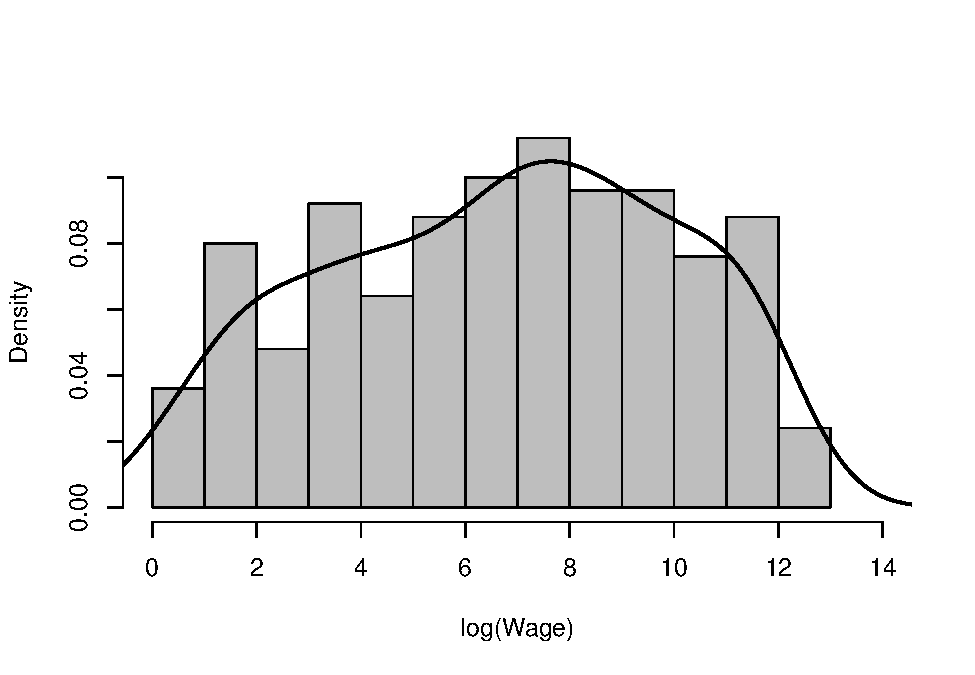
\includegraphics{assignment_1_files/figure-latex/fig_density_log_wage-1} 

}

\caption{\label{fig:figs}Kernel density plot of predicted $log(Wage)$ of the unemployed.}\label{fig:fig_density_log_wage}
\end{figure}

\clearpage

\hypertarget{question-2-earnings-and-schooling}{%
\subsection{Question 2: Earnings and
Schooling}\label{question-2-earnings-and-schooling}}

The same researcher is interested in estimating the causal effect of
schooling on earnings for employed individuals only. As a consequence,
she performs the subsequent analysis on the (sub)sample of employed
individuals.

\textbf{(a) Discuss the estimation of the causal effect of schooling on
earnings by OLS. In particular, address whether or not it is plausible
that regularity conditions for applying OLS are satisfied.}

It is not plausible that the regularity conditions are satisfied. In
particular, an observable such as an individual's \textbf{ability} might
be correlated with the wage, but also with the decision to live close to
a school. Hence, the estimates suffer from endogeneity.

\textbf{(b) The researcher has collected data on two potential
instrumental variables subsidy and distance for years of schooling.}

\begin{itemize}
\tightlist
\item
  \textbf{distance measures the distance between the school location and
  the residence of the individual while at school-going age.}
\item
  \textbf{subsidy is an indicator depending on regional subsidies of
  families for covering school expenses.}
\end{itemize}

The researcher has the option to use only distance as an instrumental
variable, or to use only the instrumental variable subsidy, or to use
both distance and subsidy as instrumental variables. Perform
instrumental variables estimation for these three options. Which option
do you prefer? Include in your answer the necessary analyses and numbers
on which you base your choice.

\begin{Shaded}
\begin{Highlighting}[]
\NormalTok{firstoption <-}\StringTok{ }\KeywordTok{ivreg}\NormalTok{(}\DataTypeTok{data =}\NormalTok{ data, }\DataTypeTok{formula =} 
\NormalTok{                         logWage }\OperatorTok{~}\StringTok{ }\NormalTok{age }\OperatorTok{+}\StringTok{ }\NormalTok{age2 }\OperatorTok{+}\StringTok{ }\NormalTok{schooling }\OperatorTok{|}\StringTok{ }\NormalTok{distance }\OperatorTok{+}\StringTok{ }\NormalTok{age }\OperatorTok{+}\StringTok{ }\NormalTok{age2)}

\NormalTok{secondoption <-}\StringTok{ }\KeywordTok{ivreg}\NormalTok{(}\DataTypeTok{data =}\NormalTok{ data, }\DataTypeTok{formula =}
\NormalTok{                          logWage }\OperatorTok{~}\StringTok{ }\NormalTok{age }\OperatorTok{+}\StringTok{ }\NormalTok{age2 }\OperatorTok{+}\StringTok{ }\NormalTok{schooling }\OperatorTok{|}\StringTok{ }\NormalTok{subsidy }\OperatorTok{+}\StringTok{ }\NormalTok{age }\OperatorTok{+}\StringTok{ }\NormalTok{age2)}

\NormalTok{thirdoption <-}\StringTok{ }\KeywordTok{ivreg}\NormalTok{(}\DataTypeTok{data =}\NormalTok{ data, }\DataTypeTok{formula =}
\NormalTok{                          logWage }\OperatorTok{~}\StringTok{ }\NormalTok{age }\OperatorTok{+}\StringTok{ }\NormalTok{age2 }\OperatorTok{+}\StringTok{ }\NormalTok{schooling }\OperatorTok{|}\StringTok{ }\NormalTok{subsidy }\OperatorTok{+}\StringTok{ }\NormalTok{distance }\OperatorTok{+}\StringTok{ }\NormalTok{age }
                     \OperatorTok{+}\StringTok{ }\NormalTok{age2)}
\end{Highlighting}
\end{Shaded}

\begin{Shaded}
\begin{Highlighting}[]
\KeywordTok{stargazer}\NormalTok{(firstoption, secondoption, thirdoption, }\DataTypeTok{font.size =} \StringTok{"small"}\NormalTok{, }
          \DataTypeTok{style =} \StringTok{"AER"}\NormalTok{, }
          \DataTypeTok{header =}\NormalTok{ F)}
\end{Highlighting}
\end{Shaded}

\begin{table}[!htbp] \centering 
  \caption{} 
  \label{} 
\small 
\begin{tabular}{@{\extracolsep{5pt}}lccc} 
\\[-1.8ex]\hline 
\hline \\[-1.8ex] 
\\[-1.8ex] & \multicolumn{3}{c}{logWage} \\ 
\\[-1.8ex] & (1) & (2) & (3)\\ 
\hline \\[-1.8ex] 
 age & $-$0.192 & $-$0.233 & $-$0.229 \\ 
  & (0.587) & (0.546) & (0.547) \\ 
  & & & \\ 
 age2 & $-$0.014 & $-$0.013 & $-$0.013 \\ 
  & (0.010) & (0.009) & (0.009) \\ 
  & & & \\ 
 schooling & 0.470 & 0.401$^{***}$ & 0.408$^{***}$ \\ 
  & (0.299) & (0.106) & (0.102) \\ 
  & & & \\ 
 Constant & 22.700$^{**}$ & 23.700$^{***}$ & 23.600$^{***}$ \\ 
  & (9.700) & (8.520) & (8.530) \\ 
  & & & \\ 
Observations & 416 & 416 & 416 \\ 
R$^{2}$ & 0.786 & 0.799 & 0.798 \\ 
Adjusted R$^{2}$ & 0.784 & 0.798 & 0.797 \\ 
Residual Std. Error (df = 412) & 1.610 & 1.560 & 1.560 \\ 
\hline \\[-1.8ex] 
\textit{Notes:} & \multicolumn{3}{l}{$^{***}$Significant at the 1 percent level.} \\ 
 & \multicolumn{3}{l}{$^{**}$Significant at the 5 percent level.} \\ 
 & \multicolumn{3}{l}{$^{*}$Significant at the 10 percent level.} \\ 
\end{tabular} 
\end{table}

We consider that the second option, to include only subsidy as an
instrument, is the best option. The reason is that distance is unlikely
to satisfy the exclusion restriction: distance is (to a certain extent)
an endogenous variable: wealthier (or more able) parents may choose to
live closer to school, and invest more in the education of their
children (or genetically transmit ability). Since a potentially
endogenous instrument must not be used as such, we prefer the estimates
in equation 2. However, we see that the results show that distance has
no predictive power in schooling, thus showing that the endogeneity is
very small. Conditional on subsidy being a good instrument, then, the
potential endogeneity does not substantially changes the estimates of
schooling on earnings.

\begin{enumerate}
\def\labelenumi{(\alph{enumi})}
\setcounter{enumi}{2}
\tightlist
\item
  Compare the IV estimates with the OLS outcomes. Under which conditions
  would you prefer OLS over IV? Perform a test and use the outcome of
  the test to support your choice between OLS and IV. Motivate your
  choice.
\end{enumerate}

We first observe that the OLS estimate \(\beta =\) 0.216 is about half
the magnitude of the IV-estimate. This means that the bias generated by
OLS likely \emph{downplays} the actual effect (if the IV estimates
satisfy the exclusion restriction). In case we would not trust the IV
assumptions, we would prefer to trust the (conservative) estimate that
downplays the effect, i.e.~the OLS estimates. We can test whether the
OLS estimates are substantially different from the IV estimates by
conducting a Hausman test:

\begin{Shaded}
\begin{Highlighting}[]
\NormalTok{hoi <-}\StringTok{ }\KeywordTok{summary}\NormalTok{(}
\NormalTok{    secondoption, }
        \DataTypeTok{diagnostics=}\OtherTok{TRUE}\NormalTok{)}

\NormalTok{hoi}\OperatorTok{$}\NormalTok{diagnostics}
\end{Highlighting}
\end{Shaded}

\begin{verbatim}
##                  df1 df2 statistic  p-value
## Weak instruments   1 412     43.32 1.42e-10
## Wu-Hausman         1 411      3.63 5.73e-02
## Sargan             0  NA        NA       NA
\end{verbatim}

The null hypothesis in the Hausman test is exogeneity of the
\emph{schooling} variable. As becomes clear, the null hypothesis is
marginally rejected, implying the \emph{schooling} is endogenous, but
only marginally so. Hence, we would prefer to trust the IV estimates in
this case.

\end{document}
